% Name und persönliche Daten nur auf DECKBLATT und EIDESSTATTLICHER ERKLÄRUNG
% DECKBLATT, SPERRVERMERK, VORWORT ohne Seitenzahlen
% INHALTSVERZ., AUFGABENSTELLUNG, VERZEICHNISSE römische Nummerierung (I, II, III)
% ALLES ANDERE arabisch (1, 2, 3)

% DIN A4
% Oben 		= 2,5 cm
% Unten 	= 2,5 cm
% Links 	= 3,0 cm
% Rechts 	= 2,5 cm

% Arial 11pt, Times New Roman 12pt
% Zeilenabstand: einfach -1.5
% Blocksatz mit Silbentrennung
% Überschriften im Text abheben (fett oder so)
% Zitierstil: IEEE
% Bild 1: <Beschreibung> (unten)
% Tabelle 1: <Beschreibung> (oben)
% caption links und label in caption Fett!


%%%%%%%%%%%%%%%%%%%%%%%%%%%%%%%%%%%%%
%%% BIBLIOTHEKEN %%%%%%%%%%%%%%%%%%%%
%%%%%%%%%%%%%%%%%%%%%%%%%%%%%%%%%%%%%

\documentclass[a4paper,12pt,headsepline]{scrartcl}

\usepackage[utf8]{inputenc} 	% utf-8 encoding
\usepackage{graphicx} 			% Grafiken
\usepackage[ngerman]{babel} 	% deutsch als Hauptsprache
\usepackage[right]{eurosym} 	% Eurozeichen
\usepackage{fontspec} 			% Zeichenencoding
\usepackage{lmodern}			% flüssigere Schrift
\usepackage{longtable} 			% mehrseitige Tabellen
\usepackage[left=3cm,right=2.5cm,top=2.5cm,bottom=2.5cm,includeheadfoot]{geometry}
								% Seitenränder
\usepackage{fancybox} 			% Paket für Boxen im Text
\usepackage{url} 				% bricht lange URLs "schön" um
\usepackage[dvipsnames,table]{xcolor}	% Textfarben (dvipsnames = mehr farben!)
\usepackage{amsmath,amsthm,amssymb,amsfonts}
								% Mathe Formeln, Zeichen etc.
\usepackage[hidelinks]{hyperref} 			% erzeugt Inhaltsverzeichnis mit Querverweisen zu den Abschnitten (PDF Version)
\usepackage{fancyhdr} 			% Kopf- Fußzeilen
%\usepackage{array} 			% für Tabellen
\usepackage[onehalfspacing]{setspace} 
								% Paket für Zeilenabstand
\usepackage{caption}			% extended captions (fettes label)
\usepackage{makeidx} 			% extended index
\usepackage[newfloat]{minted} 			% code Blöcke
\usepackage[backend=biber, sorting=none, citestyle=ieee]{biblatex}

\usepackage[german]{nomencl}
\usepackage{acronym}
\usepackage{tabularx}
\usepackage{multirow}
\usepackage{float}				% Bilder mit [H] genau dort einordnen wo sie hin sollen
%\usepackage{dblfloatfix}
%\usepackage[titles]{tocloft} 	% Für Formeln und Formelverzeichnis
%\usepackage{floatflt} 			% floatende Bilder ermöglichen
\usepackage{booktabs}			% Toprule etc.
\usepackage{subcaption}			% Bilder nebeneinander
\usepackage{tocloft}			% for cftdot command
\usepackage[export]{adjustbox}	% adjust alignment for images
\usepackage{pdfpages}

%%%%%%%%%%%%%%%%%%%%%%%%%%%%%%%%%%%%%
%%% EINSTELLUNGEN %%%%%%%%%%%%%%%%%%%
%%%%%%%%%%%%%%%%%%%%%%%%%%%%%%%%%%%%%

\graphicspath{ {abb/} }

%% no dots in toc
%\renewcommand{\cftdot}{}

%% for dots
\renewcommand{\cftsecleader}{\cftdotfill{\cftdotsep}} % for sections
%\renewcommand{\cftchapleader}{\cftdotfill{\cftdotsep}} % for chapters
%\renewcommand{\cftpartleader}{\cftdotfill{\cftdotsep}} % for parts

%% Sektion Einstellungen
%\titleformat{\section}
%{\normalfont\sffamily\huge\bfseries\color{black}}
%{\thesection}{20pt}{\Huge}
%\titleformat{\subsection}
%{\normalfont\sffamily\huge\bfseries\color{black}}
%{\thesubsection}{20pt}{\Huge}

%% Sektions gleicher Font wie Text
\addtokomafont{disposition}{\rmfamily}
\setkomafont{title}{\huge\bfseries}
\addtokomafont{titlehead}{\LARGE\centering}

% label in captions fett, caption links aligned! 
\captionsetup{labelfont=bf, justification=raggedright, singlelinecheck=false}

% Pfad für bilder setzen
%\graphicspath{./abb/}

% Neuer Absatz ohne Ausrückung
\setlength{\parindent}{0pt}
%\geometry{left=3cm, right=2.5cm, top=2.5cm, bottom=2.5cm}

% Farben definieren für CODE
\definecolor{codeGreenDark}{HTML}{1f9109}
\definecolor{codeGreenMint}{HTML}{00e061}
\definecolor{codeGray}{HTML}{a3a3a3}
\definecolor{codePurple}{HTML}{c247ff}
\definecolor{codeOrange}{HTML}{e39b00}
\definecolor{codeDarkGray}{HTML}{303030}
\definecolor{codeBgColor}{HTML}{f2f2f2}

\definecolor{imageFrameGray}{HTML}{bfbfbf}

% Farben Table
\definecolor{tableHeadColor}{HTML}{e0e0e0}
\definecolor{tableRowColor}{HTML}{f0f0f0}

% Farben definieren für TEXT
\definecolor{txtRed}{HTML}{ff0000}
\definecolor{applegreen}{rgb}{0.55, 0.71, 0.0}
\definecolor{safetyorange}{rgb}{1.0, 0.4, 0.0}

%%%%%%%%%%%%%%%%%%%%%%%%%%%%%%%%%%%%%
%%% SYMBOLVERZEICHNIS %%%%%%%%%%%%%%%
%%%%%%%%%%%%%%%%%%%%%%%%%%%%%%%%%%%%%

% Punkte zw. Abkürzung und Erklärung
\setlength{\nomlabelwidth}{.20\hsize}
\renewcommand{\nomlabel}[1]{#1 \dotfill}
% Zeilenabstände verkleinern
\setlength{\nomitemsep}{-\parsep}


%% eigene Kopfzeilen und Fußzeilen
\fancypagestyle{contents}{%
	\fancyhf{} 								% alle Kopf- und Fußzeilenfelder bereinigen
	\fancyhead[L]{\nouppercase{\leftmark}} 	% Kopfzeile links
	\fancyhead[C]{} 						% zentrierte Kopfzeile
	\fancyhead[R]{\thepage} 				% Kopfzeile rechts
	\renewcommand{\headrulewidth}{0.4pt} 	% obere Trennlinie
} % eigener Seitenstil für Inhalte

\fancypagestyle{preamble}{%
	\fancyhf{} 								% alle Kopf- und Fußzeilenfelder bereinigen
	\fancyhead{} 							% keine Kopfzeile
	\fancyfoot[C]{\thepage} 				% Kopfzeile rechts
	\renewcommand{\headrulewidth}{0pt} 	% obere Trennlinie
} % eigener Seitenstil für Preambles

%%\bibliographystyle{IEEEtran}
% Bibliographie
\addbibresource{ref.bib}
\bibliography{ref}

% Inhaltsverzeichnis
\makeindex

% Abkürzungsverzeichnis LiveTex Version
\makenomenclature

%% table of contents setup
%\setlength\cftparskip{\tocspacing}
\setlength\cftbeforesecskip{0pt}
%\setlength\cftaftertoctitleskip{2pt}

%\newcommand{\indexesspacing}{\cftbeforesecskip}
\newcommand{\indexesspacing}{\cftbeforesecskip}

\setlength\cftbeforesubsecskip{\indexesspacing}
\setlength\cftbeforesubsubsecskip{\indexesspacing}
\setlength\cftbeforefigskip{\indexesspacing}
%\setlength\cftbeforesubfigskip{\indexesspacing}
\setlength\cftbeforetabskip{\indexesspacing}
%\setlength\cftbeforesubtabskip{\indexesspacing}

%%%%%%%%%%%%%%%%%%%%%%%%%%%%%%%%%%%%%
%%% LISTINGS/CODE SETUP %%%%%%%%%%%%%
%%%%%%%%%%%%%%%%%%%%%%%%%%%%%%%%%%%%%
\newenvironment{code}{\captionsetup{type=listing}}{}
\SetupFloatingEnvironment{listing}{name=Quellcode, listname=Quellcodeverzeichnis}

%\renewcommand{\listoflistings}{%
%	\cleardoublepage
%	\addcontentsline{toc}{chapter}{\listoflistingscaption}%
%	\listof{listing}{\listoflistingscaption}%
%}

\begin{document}
	% defined commands and variables

\newcommand{\myparagraph}[1]{\paragraph{#1}\mbox{}\\}

\newcommand{\gloss}[2]{\textbf{#1}\\#2\newparagraph}

\newcommand{\inquote}[1]{
	\glqq{#1}\grqq{}
}

\newcommand{\mkred}[1]{
	\textcolor{red}{#1}
}

\newcommand{\source}[1]{\caption*{ {\small \textbf{Quelle}: {#1}} } }

\newcommand{\quoting}[2]{
	\begin{quote}
		\glqq\textit{#1}\grqq
	\end{quote}
	\begin{flushright}
		\texttwelveudash #2
	\end{flushright}
}

\newcommand{\codeinline}[1]{
	{\bfseries\small\texttt{#1}}
}

\newcommand{\codefull}[4]{
	\begin{code}
		\captionof{listing}{#2}
		\label{#1}
		\inputminted[breaklines, bgcolor=codeBgColor, linenos]{#3}{#4}
%		\caption{#2}
	\end{code}
}

%%% LABEL ALWAYS AFTER CAPTION %%%
\newcommand{\image}[4][]{
	\begin{figure}[H]
		%
		\centering
		%\includegraphics[width=1\textwidth]{images/RIFB.png}
		%\includegraphics[height=10cm, keepaspectratio=true]{#1}
		\includegraphics[width=\ifthenelse{\equal{#1}{}}{1\textwidth}{#1}, keepaspectratio=true]{#2}
		\caption{#4}
		\label{#3}
	\end{figure}
}

\newcommand{\doublefigure}[6]{
	\begin{figure}[H]
		\centering
		\begin{subfigure}[b]{.5\textwidth}
			\centering
			%\includegraphics[width=0.9\textwidth]{#1}
			\includegraphics[height=10cm]{#1}
			\caption{#2}
		\end{subfigure}%
		\begin{subfigure}[b]{.5\textwidth}
			\centering
			%\includegraphics[width=0.9\textwidth]{#3}
			\includegraphics[height=10cm]{#3}
			\caption{#4}
		\end{subfigure}
		\caption{#5}
		\label{#6}
	\end{figure}
}

\newcommand{\newparagraph}{\\[12pt]}
	\rowcolors{1}{tableRowColor}{}
	
	%%%%%%%%%%%%%%%%%%%%%%%%%%%%%%%%%%%%%
	%%% DECKBLATT %%%%%%%%%%%%%%%%%%%%%%%
	%%%%%%%%%%%%%%%%%%%%%%%%%%%%%%%%%%%%%
	
	\pagestyle{empty}
	
	\singlespacing
	\thispagestyle{empty}

%\begin{figure}[H]
%	\centering
%	\begin{subfigure}[b]{.45\textwidth}
%		\centering
%		%\includegraphics[width=0.9\textwidth]{#1}
%		\includegraphics[width=0.6\textwidth,left]{logo1.png}
%	\end{subfigure}
%	\begin{subfigure}[b]{.45\textwidth}
%		\centering
%		%\includegraphics[width=0.9\textwidth]{#3}
%		\includegraphics[width=0.55\textwidth,right]{logo_htw_small.png}
%	\end{subfigure}
%\end{figure}

\begin{verbatim}
\end{verbatim}

\begin{center}
\Large{Hochschule für Technik und Wirtschaft Berlin}\\
\end{center}

\begin{center}
\Large{Fachbereich für Ingenieurwissenschaften - Technik und Leben}
\end{center}
\begin{verbatim}
\end{verbatim}
\begin{center}
\doublespacing
\textbf{\LARGE{Bachelorarbeit}}\\
\singlespacing
\begin{verbatim}
\end{verbatim}
\textbf{{im Studiengang Ingenieurinformatik}}
\end{center}
\begin{verbatim}
\end{verbatim}
\begin{center}

\end{center}
\begin{verbatim}
\end{verbatim}
\begin{flushleft}
\begin{tabular}{llll}
\hiderowcolors
\textbf{Thema} & & TITEL &\\
& & \\
\textbf{vorgelegt von} & & Max Mustermann& \\
& & \\
\textbf{Datum} & & Berlin, 19. September 2021 &\\
& & \\
\textbf{Erstgutachter} & & Prof. Dr.-Ing. Bla &\\
\textbf{Zweitgutachter} & & Bla Bla &\\
\end{tabular}
\end{flushleft}

	\newpage
	\onehalfspacing
	
	\textcolor{gray}{\textit{Diese Seite wurde absichtlich frei gelassen}}
	\begin{verbatim}
	\end{verbatim}
	\newpage
	
	%Vorwort
	\section*{Vorwort}
Die vorliegende Bachelorarbeit entstand im Unternehmen ...
	\newpage
	
	%Sperrvermerk
	\section*{Sperrvermerk}
Die vorliegende Bachelorarbeit mit dem Titel \textbf{TITEL} enthält vertrauliche Daten des Unternehmens \textbf{UNTERNEHMEN}.\\

Diese Arbeit darf Dritten, mit Ausnahme des Erst- und Zweitgutachters und befugten Mitgliedern des Prüfungsausschusses, ohne ausdrückliche Zustimmung des Unternehmens und des Verfassers nicht zugänglich gemacht werden.\\

Eine Vervielfältigung und Veröffentlichung der Bachelorarbeit ohne vorherige Genehmigung ist auch in Auszügen nicht erlaubt. 
	\newpage
	
	%%%%%%%%%%%%%%%%%%%%%%%%%%%%%%%%%%%%%
	%%% VERZEICHNISSE %%%%%%%%%%%%%%%%%%%
	%%%%%%%%%%%%%%%%%%%%%%%%%%%%%%%%%%%%%
	
	\pagestyle{preamble}
	
	% Inhaltsverzeichnis
	\setcounter{page}{1}
	\pagenumbering{Roman}
	\tableofcontents
	\newpage
	
	% Abbildungsverzeichnis
	\addcontentsline{toc}{section}{Abbildungsverzeichnis}
	\listoffigures
	\newpage
	
	% Tabellenverzeichnis
	\addcontentsline{toc}{section}{Tabellenverzeichnis}
	\listoftables
	\newpage
	
	%	% Formelverzeichnis
	%	\addcontentsline{toc}{section}{Formelverzeichnis}
	%	\newcommand{\listequationsname}{Formelverzeichnis}
	%	\newlistof{myequations}{equ}{\listequationsname}
	%	\newcommand{\myequations}[1]{%
	%		\addcontentsline{equ}{myequations}{\protect\numberline{\theequation}#1}\par}
	%	\listofmyequations
	%	\newpage
	
	% Quellcodeausschnittverzeichnis
	\addcontentsline{toc}{section}{Quellcodeverzeichnis}
%	\listoflistings
	\listof{listing}{Quellcodeverzeichnis}
	\newpage

	
	% Abkürzungsverzeichnis
	\section*{Abkürzungsverzeichnis}\label{abkuerzung}
	\addcontentsline{toc}{section}{Abkürzungsverzeichnis}
	% \acro{kürzel}[kurzform]{langform}
	\textbf{Allgemeine technische Abkürzungen}
\begin{acronym}[JSONP]\itemsep0pt
	\acro{CSS}{Cascading Style Sheets}
	\acro{JS}{JavaScript}
	\acro{JSON}{JavaScript Object Notation}
	\acro{HTML}{Hypertext Markup Language}
	\acro{UI}{User Interface}
	\acro{API}{Application Programming Interface}
	\acro{REST}{Representational State Transfer}
	\acro{DOM}{Document Object Model}
	\acro{RWD}{Responsive Webdesign}
	\acro{QA}{Quality Assurance (Qualitätssicherung)}
\end{acronym}

\textbf{Allgemeine sprachliche Abkürzungen}
\begin{acronym}[JSONP]\itemsep0pt
 	\acro{d.h.}{das heißt}
	\acro{z.B.}{zum Beispiel}
	\acro{bspw.}{beispielsweise}
	\acro{u.a.}{unter anderem}
	\acro{bzw.}{beziehungsweise}
\end{acronym}

\textbf{Spezifische Abkürzungen}
\begin{acronym}[JSONP]\itemsep0pt
	\acro{BS}{Bullshit}
\end{acronym}
	\newpage
	
%	% Symbolverzeichnis
%	\addcontentsline{toc}{section}{Symbolverzeichnis}
%	\nomenclature{$v$}{Geschwindigkeit}
%	\printnomenclature
%	\newpage

	% Glossar
	\addcontentsline{toc}{section}{Glossar}
	\section*{Glossar}

\gloss{Sitzungstoken (\textit{session token})}{Art der Identifikation eines Benutzers für eine Sitzung.}
%\gloss{Swagger}{Dokumentationstool für APIs.}
%\gloss{Mock-Up}{Ein Mock-Up ist ein Vorführmodell für ein Produkt.}
%\gloss{Propdrilling}{Erklärung des Begriffes}
\gloss{DOM}{Das Document-Object-Model ist die Schnittstelle zwischen HTML und JavaScript, welche die dynamische Manipulation von HTML-Elementen durch JavaScript erlaubt.}
% https://wiki.selfhtml.org/wiki/JavaScript/DOM#DOM-Manipulation
\gloss{Memoisation}{Die Zwischenspeicherung eines Rückgabewerts, um die Geschwindigkeit eines Programms zu beschleunigen.}
\gloss{Rückruffunktion (\textit{callback function})}{Funktion, die unter bestimmten Bedingungen und mit Parametern zu einem Zeitpunkt aufgerufen wird.}
\gloss{Microservice}{Eigenständige Softwarekomponente eines Systems, die eine bestimmte Funktion übernimmt. Das System ist in mehrere Microservices unterteilt.}
\gloss{JSX}{Eigene Sprache vom JavaScript-Framework React zum Kombinieren von HTML- und JS-Code um dynamisch die Benutzeroberfläche zu manipulieren.}
\gloss{JavaScript-Objekt}{Ein Datentyp in JavaScript aus der Kategorie Schlüssel-Werte-Sammlung.}
\gloss{Stylesheet-Sprache}{Formale Sprache in der Informationstechnik zum Verändern des Erscheinungsbilds einer Benutzeroberfläche.}
	\newpage
	
	\addcontentsline{toc}{section}{Abstract}
	\section*{Abstract}

	\newpage
	
	%%%%%%%%%%%%%%%%%%%%%%%%%%%%%%%%%%%%%
	%%% HAUPTTEIL %%%%%%%%%%%%%%%%%%%%%%%
	%%%%%%%%%%%%%%%%%%%%%%%%%%%%%%%%%%%%%
	
	\pagestyle{contents}
	
	\renewcommand{\sectionmark}[1]{\markright{#1}}
	%\lhead{\fancyplain{}{\rightmark }}
	\fancyhead[L]{\nouppercase{\leftmark}}
	\pagenumbering{arabic}
	
%	\fancyhead[L]{Einleitung}
%	\input{pages/2_einleitung}
%	\newpage
%
%	\input{pages/3_hauptteil}
%	\newpage
%	
%	\fancyhead[L]{Zusammenfassung und Ausblick}
%	\input{pages/4_zusammenfassung}
%	\newpage

	\section{Kapitel 1}
Codebeispiel in \autoref{code:useEffect-sample}

\codefull{code:useEffect-sample}{Implementierung des \codeinline{useEffect}-Hooks}{jsx}{code/useEffect-sample.jsx}

% Mit extra optionen
\codefull[firstline=4, lastline=6]{code:useEffect-sample-options}{Implementierung des \codeinline{useEffect}-Hooks}{jsx}{code/useEffect-sample.jsx}

Abbildung in \autoref{img:redux-saga-flow}

\begin{figure}[H]
	\centering
	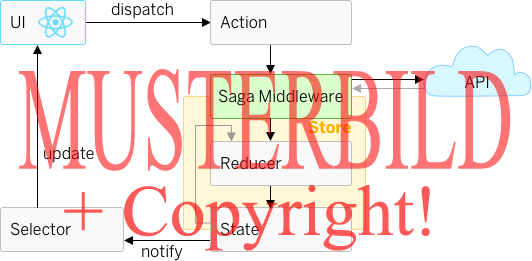
\includegraphics[height=6cm]{redux-saga-flow}
	\caption{Datenfluss mit Redux und Redux-Saga als Bibliothek}
	\label{img:redux-saga-flow}
\end{figure}

Abbildungen nebeneinander mit Frame in \autoref{img:tabl}

\begin{figure}[H]
	\centering
	\begin{subfigure}[b]{.45\textwidth}
		\centering
		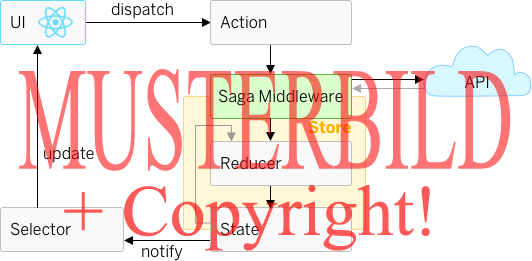
\includegraphics[width=1.0\textwidth, cframe=imageFrameGray]{redux-saga-flow}
		\caption{Kopfleiste}
		\label{img:tablet-head}
	\end{subfigure}
	\begin{subfigure}[b]{.45\textwidth}
		\centering
		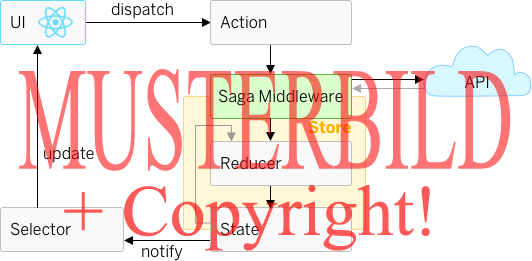
\includegraphics[width=1.0\textwidth, cframe=imageFrameGray]{redux-saga-flow}
		\caption{Filtermenü}
		\label{img:tablet}
	\end{subfigure}
	\caption{Vorführmodell des Statistikfilters für Tabletgeräte}
	\label{img:tabl}
\end{figure}

Tabelle in \autoref{tab:sec-verification-runs}

\begin{longtable}[c]{p{1cm} p{9cm} p{4cm}} 
	\hiderowcolors
	\caption{Ablauf und Ergebnis der Testszenarien für die Sicherheitsanforderung}
	\label{tab:sec-verification-runs}\\
	\bottomrule
	\showrowcolors
	\rowcolor{tableHeadColor}
	\textbf{ID} & \textbf{Ablauf} & \textbf{Ergebnis} \\
	%\midrule
	\hline
	\endfirsthead
	%
	\hiderowcolors
	\multicolumn{3}{c}{{\textit{Tabelle \thetable\ von letzter Seite fortgesetzt} }} \\
	\endhead
	%
	%\hline
	\multicolumn{3}{r}{\textit{Fortsetzung auf nächster Seite}} \\
	\endfoot
	%\hline
	\endlastfoot
	\showrowcolors
	%
	TS1 &
	\begin{minipage}[t]{9cm}
		\begin{enumerate}
			\item Testnutzer erhält Rolle für sein Profil
			\item Testnutzer meldet sich im Netzwerk mit seinem Profil an
			\item Testnutzer ruft Webanwendung auf
		\end{enumerate}
	\end{minipage}  & 
	\begin{minipage}[t]{4cm}
		\textcolor{applegreen}{$ \checkmark $ } bestanden
	\end{minipage}  \\ 
	TS2 &
	\begin{minipage}[t]{9cm}
		\begin{enumerate}
			\item Testnutzer meldet sich im Netzwerk mit seinem Profil an
			\item Testnutzer ruft Webanwendung auf
		\end{enumerate}
	\end{minipage}  & 
	\begin{minipage}[t]{4cm}
		\textcolor{applegreen}{$ \checkmark $ } bestanden
	\end{minipage}  \\ 
	TS3 &
	\begin{minipage}[t]{9cm}
		\begin{enumerate}
			\item Testnutzer erhält Rolle für sein Profil
			\item Testnutzer ruft Webanwendung auf
		\end{enumerate}
	\end{minipage}  & 
	\begin{minipage}[t]{4cm}
		\textcolor{applegreen}{$ \checkmark $ } bestanden
	\end{minipage}  \\ 
	TS4 &
	\begin{minipage}[t]{9cm}
		\begin{enumerate}
			\item Testnutzer erhält Rolle für sein Profil
			\item Testnutzer meldet sich im Netzwerk mit seinem Profil an
			\item Testnutzer wartet bis Sitzung nicht mehr gültig ist
			\item Testnutzer besucht Webanwendung
		\end{enumerate}
	\end{minipage}  & 
	\begin{minipage}[t]{4cm}
		\textcolor{applegreen}{$ \checkmark $ } bestanden
	\end{minipage}  \\ 
	TS5 &
	\begin{minipage}[t]{9cm}
		Alle Schritte aus TS4 werden durchlaufen und folgende Schritte werden danach ausgeführt:
		\begin{enumerate}
			\item Sitzung wird invalidiert/deaktiviert (entweder durch Entfernen des Sitzungstoken-Cookies, oder durch Ablaufen der Sitzung)
			\item Testnutzer lädt neue Statistiken
		\end{enumerate}
	\end{minipage}  & 
	\begin{minipage}[t]{4cm}
		\textcolor{applegreen}{$ \checkmark $ } bestanden
	\end{minipage}  \\
	\bottomrule     
\end{longtable}

Refernz auf \cite{augsten_2017_was}.
	\newpage
	
	%%%%%%%%%%%%%%%%%%%%%%%%%%%%%%%%%%%%%
	%%% LITERATURVERZEICHNIS %%%%%%%%%%%%
	%%%%%%%%%%%%%%%%%%%%%%%%%%%%%%%%%%%%%
	
	\addcontentsline{toc}{section}{Literaturverzeichnis}
	\renewcommand\refname{Literaturverzeichnis}
	\fancyhead[L]{Literaturverzeichnis}
	\printbibliography
	\newpage
	
	%	 Anhang
	\newpage
	\addcontentsline{toc}{section}{Anhang}
	\fancyhead[L]{Anhang} %Kopfzeile links
	\section*{Anhang}
	
	% Eidesstattliche Erklärung
	\newpage
	\addcontentsline{toc}{section}{Eidesstattliche Erklärung}
	\section*{Eidesstattliche Erklärung}
\thispagestyle{empty}

\begin{verbatim}
\end{verbatim}

Ich erkläre hiermit an Eides statt, dass

\begin{itemize}
	\item ich die vorliegende wissenschaftliche Arbeit selbständig und ohne unerlaubte Hilfe angefertigt habe,
	\item ich andere als die angegebenen Quellen und Hilfsmittel nicht benutzt habe,
	\item ich die den benutzten Quellen wörtlich oder inhaltlich entnommenen Stellen als solche kenntlich gemacht habe,
	\item die Arbeit in gleicher oder ähnlicher Form noch keiner anderen Prüfbehörde vorgelegen hat.
\end{itemize}

\vspace{5cm}
\textbf{\today}
\hspace{7cm}
\textbf{Max Mustermann}

%\begin{displaymath}
%% use packages: array
%\begin{array}{ll}
%Ort, Datum:~~~~~~~~~~~~~~~~~~~~~~~~~~~~~~~~~~~~~~~~~~
%&Unterschrift:~~~~~~~~~~~~~~~~~~~~~~~~~~~~~~~~~~~~~~~~~~
%\end{array}
%\end{displaymath}
	
\end{document}